\title{Inferencing From Bayesian Networks\\Lab 5}
\author{
Aditya Gupta \\
\and
Milan Chaudhary
}
\date{\today}

\documentclass[12pt]{article}

\usepackage{tikz}
\usetikzlibrary{datavisualization}

\begin{document}
\maketitle

\section{Introduction}
In this Lab exercise .... .... ... 

\section{Variable Elimination}
In this section of program, first a container with all the conditional probability tables from each node instantiated by the evidence varaibles were collected. Then for each evidence variable, all the factors with that variable in it was collected and joined together. This process was repeated until all hidden variables were joined (and summed). The result was thus the required row (after normalization) of the table formed from joining all the remaining factors.

\subsection{Reduce}
For each row the index (in binary) was masked with 1 for all non-evidence variables. This leaves behind only the evidence variables and all must thus have same transformed value since evidence are given. Thus comparison was done and required rows were collected.

\subsection{Join}
In this operation the resultant factor will have union of all variables in both the factors, further the order of the variables is important. First the common variables were collected then the remaining variables from first then second factor. Both the tables were sorted by creating weights (for common variables) and performing a stable sort (for the remaining variables). The sort involved sorting indices nstead o the whole table and then for each common value of evidence the other variables's value were taken as a block and the result were calculated block by block by two nested loops.

\subsection{Sum}
We note that for summing over a variable, the value of it only changes periodically, the period was found out and then a skipping loop summed the probabilities.

\subsection{Normalize}
The sum of the probabilities should be one, thus each was divided by the current sum.

\section{Rejection Sampling}
In this section of program, it will  n ..

\subsection{Convergence of the probabilities as function of\\ number of samples generated}
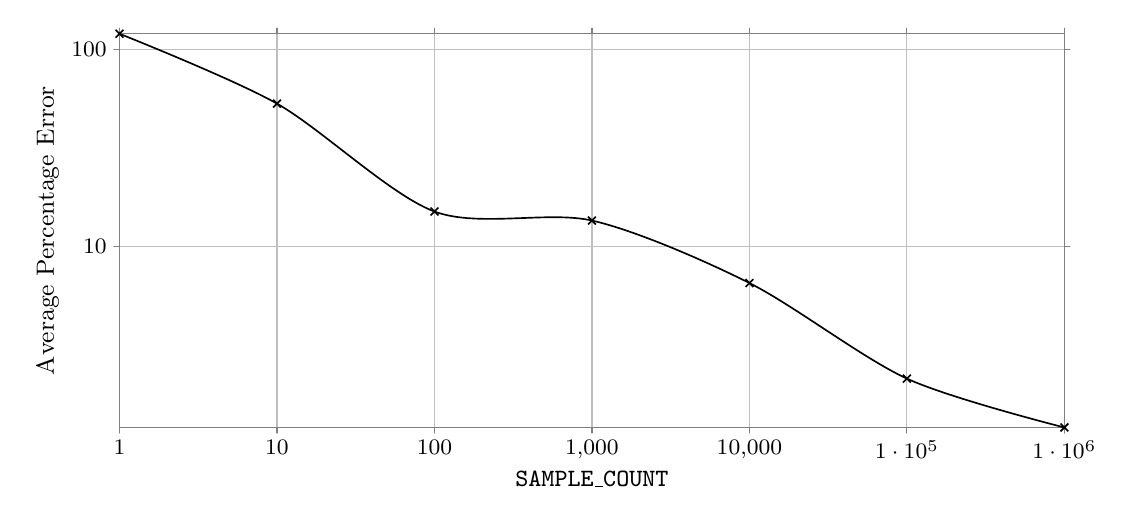
\begin{tikzpicture}
    \datavisualization [scientific axes,
    						 x axis={logarithmic,length=12cm,label=\texttt{SAMPLE\_COUNT},grid},
     						 y axis={logarithmic,length=5cm,label=Average Percentage Error,grid},
    						 visualize as smooth line=my data,
    						 my data={style={mark=x}}]
    data {
        x, y
        1, 120
        10, 53
        100, 15
        1000, 13.5
        10000, 6.5
        100000, 2.125
        1000000, 1.2
    };
\end{tikzpicture}

\end{document}
  
